\documentclass[11pt]{article}
\usepackage{fullpage}
\usepackage{comment}
\bibliographystyle{plain}
%\bibliographystyle{asa}
%\bibliographystyle{harvard}
%\bibliographystyle{apalike}


% Issues:
%  I haven't worked out a consistent notation:  when to display
%  a button's contents in bf, when to use em, etc.

% Some pictures are now out of date, such as the variable
% manipulation table.

%%%%%%%%%%%%%%%%%%%%%%%%%%%%%%%%%%%%%%%%%%%%%%%%%%%%%%%%%%%%%%%%%%%%%%

\newif\ifpdf
\ifx\pdfoutput\undefined
  \pdffalse
\else
  \pdftrue
\fi
  
\ifpdf
  \pdfoutput=1
  \usepackage[pdftex]{graphicx}  % uncomment if using graphicx
  \usepackage[pdftex]{hyperref}  % uncomment if using hyperref
\else
  \usepackage{graphicx}  % uncomment if using graphicx
  \usepackage[colorlinks=true,
    linkcolor=webgreen,
    filecolor=webbrown,
    citecolor=webgreen]{hyperref} % uncomment if using hyperref
  \definecolor{webgreen}{rgb}{0,.5,0}
  \definecolor{webbrown}{rgb}{.6,0,0}
  % dvips -z
\fi
%%%%%%%%%%%%%%%%%%%%%%%%%%%%%%%%%%%%%%%%%%%%%%%%%%%%%%%%%%%%%%%%%%%%%%

\hyphenation{XGobi}
\hyphenation{GGobi}
\hyphenation{ggobi}
\hyphenation{di-men-sion-al two--di-men-sion-al}
\input epsf
\def\Rcirc{\mbox{\small{\ooalign{\hfil\raise.07ex\hbox{\tiny R}\hfil\crcr\mathhexbox20D}}}}

\parindent 0in
\parskip 6pt

\begin {document}
\title {{\tt ggobi} Manual}
\author{
Deborah F. Swayne, AT\&T Labs -- Research \\
Di Cook, Iowa State University \\
Andreas Buja, The Wharton School, University of Pennsylvania \\
Duncan Temple Lang, University of California at Davis
}

\date{September 2005}

\maketitle

\begin{abstract}

The GGobi software is a data visualization system with state-of-the-art
interactive and dynamic methods for the manipulation of views of
data.  It represents a significant improvement on its predecessor, XGobi,
with multiple plotting windows, more flexible color management, XML file
handling, and better portability to Windows.

The most significant change may be that ggobi is so easy to extend, either
with the addition of ``plugins'' or by embedding it in other software;
either way, it can be controlled using an API (application programming
interface).  When ggobi is embedded in R, for example, the result is a
full marriage between ggobi's direct manipulation graphical environment
and R's familiar extensible environment for statistical data analysis.

It has the same graphical functionality whether it is running
standalone or embedded in other software.  That functionality includes
2-D displays of projections of points and edges in high-dimensional
spaces, as well as scatterplot matrices, parallel coordinate, time
series plots and bar charts.  Projection tools include average shifted
histograms of single variables, plots of pairs of variables, and grand
tours of multiple variables.  Views of the data can be reshaped.
Points can be labeled and brushed with glyphs and colors.  Several
displays can be open simultaneously and linked for labeling and
brushing.  Missing data are accommodated and their patterns can be
examined.
\end{abstract}

\newpage

% I like this here, because otherwise there's no title page
\tableofcontents
\newpage

\section{Introduction}

This paper gives an overview of the layout and functionality of GGobi,
interactive graphical software for exploratory data analysis.  Readers
who are familiar with XGobi will find much that is familiar in GGobi's
design, and might want to read section \ref{slbl:xgobi} first, where
key differences between the two programs are described. There are
several papers that describe parts of the functionality existing in
both packages
\cite{BCS95,SCB97,SB98,BAHM88,CBC93,CBCH95,CB95,BCAH95c}.

You will find that you can use GGobi for simple tasks with virtually
no instruction.  All that a user needs is some cursory knowledge of
the developments in interactive statistical graphics of the last 15
years, as well as a willingness to experiment with the sample data
provided and guided by the tooltips.  In parallel with the hands-on
learning process, it is probably useful to acquire a basic
understanding of the overall layout and functionality of the system.
The greatest success is obtained by users who have gained experience
with the system and combine it with creativity and data analytic
sophistication.

We begin with a tutorial, and move on to describe GGobi in detail.

\section{Tutorial}

Several sample data files are included with the GGobi distribution, in
a directory called {\bf data,} and there you will find the file {\bf
olive.xml}, a dataset on olive oil samples from Italy \cite{FALT83}.
This data set uses an XML format.  The olive oil data consists of the
percentage composition of 8 fatty acids (palmitic, palmitoleic,
stearic, oleic, linoleic, linolenic, arachidic, eicosenoic) found in
the lipid fraction of 572 Italian olive oils. There are 9 collection
areas, 4 from southern Italy (North and South Apulia, Calabria,
Sicily), two from Sardinia (Inland and Coastal) and 3 from northern
Italy (Umbria, East and West Liguria).

The data is part of a quality control study of olive oils. It is proposed
that the olive oils from different regions have different fatty acid
signatures.

Start GGobi for the olive oils data by typing:

\begin{verbatim}
ggobi olive
\end{verbatim}

Two windows will appear, the GGobi console
and a scatterplot, as shown in Figure~\ref{fig1}.

The console has a panel of controls on the left, labeled {\bf
XYPlot}, and a variable selection region on the right.  You can see
that the scatterplot contains a 2-dimensional projection of the data,
a plot of Area vs Region.  Move the mouse to one of the variable labels
in the variable selection region, and leave it in place until the
tooltip appears, explaining how to select new variables for the
plot.   Begin to get a feeling for the data by looking at several of
the 2d plots:  Area vs palmitic, Region vs oleic, etc.

\begin{figure}[h]
%\epsfxsize 6in \centerline{\epsfbox{figures/manual1.ps}}
\hbox{\pdfimage width 3in {Figures/olive1.jpg}
      \pdfimage width 3in {Figures/olive2.jpg}
}
%\vspace{.15in} \centerline{ \parbox{6in}
\caption{Layout of a ggobi session.  The plotting window contains a
scatterplot of the Area vs Region, from the olive oils data.
}%}
\label{fig1}
\end{figure}

Next, get acquainted with the main menubar for the console by
exploring each of its menus.  Pay particular attention to the
Display, View, Interaction and Tools menus.

\begin {itemize}
\item The Display menu is the interface for opening new plotting
  windows.
\item The View menu is the interface for specifying the
  projection (1d, 2d, 3d or higher) for the current display.  (For
  some displays, such as the parallel coordinates display, there are
  no choices in the projection used, so the View menu is not
  always present.)
\item The Interaction menu is the interface for specifying the mouse
  interactions (for scaling the plot, highlighting points, and so on)
  for the current plot.
\item The Tools menu lets you open other windows to manipulate
  characteristics of the data and the view.
\end {itemize}

Using the Interaction menu, choose {\bf Identify}. Look at the buttons
inside the leftmost portion of the ggobi console. Notice that they're
contained by a frame labeled {\bf Identify,} which is the interaction mode
of the current plot.  This frame contains most of the row labeling
controls, which are described in section \ref{slbl:Identify}. Move the
cursor around the plot window using the mouse, and observe the labels
of the point closest to the cursor.  The labels for this data set show
the geographic area where the sample was taken.

Using the Display menu, open a barchart display. Notice that the new
window has a narrow white band drawn around the outside of the plotting
area:  that means that the new window is now the ``current display''
and its plot is the ``current plot.''  Click in the plotting region
of the other scatterplot to make it the current plot, and notice what
happens in the console when you alternate between the two.  Both the
controls and the variable selection region correspond to the current plot.

Now set up a plot of linoleic vs eicosenoic in the first scatterplot,
and disply Region in the barchart, and make the barchart the current
plot.  Using the Interaction menu, choose {\bf Brush.}  Look at the
buttons and menus inside the leftmost portion of the ggobi console.
Notice that they're contained by a frame labeled {\bf Brush,} which is
the view mode of the current plot.  This frame contains most of the
brushing controls, which are described in the section
\ref{slbl:Brush}.  A few of the brushing controls, though, are in the
{\bf Brush} menu in the display menubar.

The rectangle that appears in the current plot is the ``paintbrush,''
and dragging it over bars (or in a scatterplot the points) changes
their color. Change the color of the brush by opening up the {\bf
Choose color \& glyph} panel (Figure \ref{fig2}). Hold down the left
button and drag the mouse to paint the first region, then the second
and third regions, or click on the bars.  Since you're brushing in the
{\bf Transient} style, the points resume their original color when the
paintbrush no longer surrounds them.

While you brush, keep an eye on the plot of linoleic vs eicosenoic,
and notice where the painted points fall in that scatterplot (Figure
\ref{fig3}).  The oils from region 1, south Italy, are separable from
the other two regions using eicosenoic acid. Using two linked 2d plots
is one way to explore the relationship among three variables.

\begin{figure}[htp]
\begin{center}
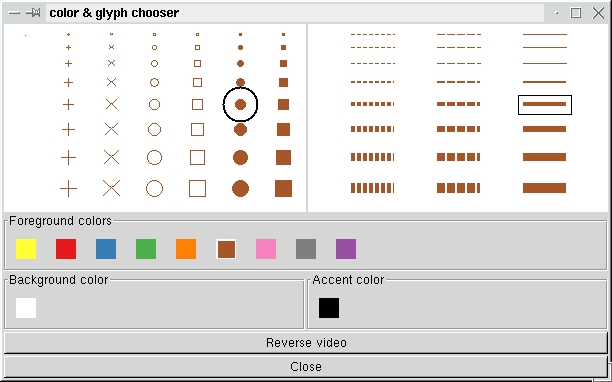
\includegraphics[width=4in]{Figures/olive-colorchoose.jpg}
\end{center}
\caption{The chooser for selecting color and glyph for painting points,
as well as type and thickness for painting lines. It also allows setting
the plot background color, and has a full color wheel for tuning the
colors.
}
\label{fig2}
\end{figure}

\begin{figure}[htp]
\hbox{\pdfimage width 3in {Figures/olive-brush1.jpg}
      \pdfimage width 3in {Figures/olive-brush2.jpg}
}
\caption{Brushing in a GGobi session. Brushing Region 1 shows that it
corresponds to a cohesive cluster in the variables linoleic and 
eicosenoic acid.
}
\label{fig3}
\end{figure}

Change to {\bf Persistent} brushing and paint the three Regions
using different colors. 

Open the {\bf Variable transformation} tool, select all of the fatty
acid variables -- either hold down the control button while selecting
them one at a time, or select the first one, then hold down the
shift button down while you select the last one.  Once they're all
highlighted, choose {\bf Standardize} in the ``Stage 2'' transformation
panel to standardize all the variables to have mean 0 and variance 1.
This tool has numerous transformations, which can be applied in sequence.
Stage 0 transformations are used to adjust variables' values so that
they're within the range of some stage 1 transformations. Stage 2
transformations allow for post-processing of stage 1 transformations,
so that the variables can be logged and then standardized, for example.

But that was just an instructive detour; click ``Reset all'' to
to turn off standardization and any other transformations you've
explored.

\begin{figure}[htp]
%\vspace{-0.5in}
%\epsfxsize 6in \centerline{\epsfbox{figures/manual1.ps}}
\pdfimage width 6in {Figures/olive-var.jpg}
%\vspace{.15in} \centerline{ \parbox{6in}
\caption{The variable manipulation panel contains basic summary 
statistics of variables. It can also be used for adding new variables
and for variable subset selection before launching multi-plot
displays.
}%}
\label{fig4}
\end{figure}

Now look at the plot of linoleic vs eicosenoic. Open up the {\bf
Color \& glyph groups ...} tool, and experiment with it:  Use the
``Shadow'' toggle buttons to have groups of points drawn in a dim
color, and then use ``Exclude shadows'' to exclude them altogether,
and ``Include shadows'' to re-include them.  (Figure \ref{fig5}).
Finally, use these controls to shadow brush the cases from geographic
region 1, and then use {\bf Exclude shadows} to remove them from
consideration.

\begin{figure}[htp]
\hbox{\pdfimage width 3in {Figures/olive-brush3.jpg}\pdfimage width 3.5in {Figures/olive-brush4.jpg}}
\caption{Toggling clusters of points on and off according to color/glyph value.}
\label{fig5}
\end{figure}

Switch into {\bf 2D Tour} using the {\bf View} menu. A column of
variable circles is added to the right of the variable toggles, one for
each selected variable.  Click on the toggle widgets for the variables
palmitoleic through arachidic to make these variables available for
touring, and toggle Region and Area out of the tour.  Click the {\bf
Reinit} button.  The tour should now include 7 variables, with one variable
circle for each.

The scrollbar at the top of the tour controls is used to adjust the
speed of the tour.  Drag it to the right to speed up the rotation.
The circle at the bottom left of the plot window displays the axes for
the tour. These can be removed by toggling the ``Show axes'' button on
the display's {\bf 2D Tour} menu.  Pause the tour when you see a
separation of the two regions (as seen in Figure \ref{fig6}).

Now you are going to use manual tour controls to sharpen up the
separation by manually changing the coefficients of the variables in
the projection.  Click on the {\bf Manip} (magenta) button below the
variable selection region of the console, and then click on linoleic
acid (a magenta circle will be seen now in the variable circle for
linoleic acid).  {\bf Oblique} is already selected in the {\bf Manual
manipulation} menu.  In the plot window, hold down any mouse
button while you drag the cursor. The coefficient corresponding to
linoleic acid will increase and decrease following the mouse, inducing
a rotation of the scattercloud.  If the axes are still showing in the
scatterplot window, the axis in magenta corresponds to the variable
you're manipulating.  Similarly rotate oleic acid and arachidic acid
in and out of the plot, with the aim of finding a projection where the
two regions are well separated (for example, Figure \ref{fig6}).
There are 5 choices of manipulation mode (unconstrained oblique,
vertical, horizontal, radial and angular) to explore.

\begin{figure}[htp]
\hbox{\pdfimage width 3in {Figures/olive-tour1.jpg}\pdfimage width 3in {Figures/olive-tour2.jpg}}
\caption{Tour plots revealing difference between regions 2 and 3 of the
olive oils.}
\label{fig6}
\end{figure}

Next use the Tools menu to open the {\bf Variable manipulation} tool
(Figure \ref{fig4}).  It contains a notebook widget which separates
the variables by type, and displays information about them in a set
of tables.  The buttons below the tables allow you to set variable
limits, add new variables, and a few other things.  Try clicking the
mouse in the table -- you can select one row of the table at a time,
or use the control and shift keys as modifiers to select more than one.
Select all the fatty acid variables, all of which are in the table
of real variables.

Open a parallel coordinates display using the {\bf Display} menu.
%Using the {\bf Selection Mode:} menu on the control
%panel select {\bf Delete} mode to remove Region and Area from the
%parallel coordinates plot. Then switch to {\bf Append} mode and add
%the remaining acid variables.
Select the first plot in the parallel coordinates display by
clicking on it, and use the {\bf Interaction} menu to switch to {\bf
Brush} mode. Choose a new color (say yellow) and large closed glyph,
and transiently paint the case with a very low value on palmitic
(Figure \ref{fig7}). This case also has a very high value for oleic
acid, and low value for linolenic acid.

\begin{figure}[htp]
\hbox{\pdfimage width 6in {Figures/olive-par.jpg}}
\caption{Brushing in a parallel coordinates display reveals an outlier in 
palmitic, oleic and linolenic acids.}
\label{fig7}
\end{figure}

Using the {\bf Color \& glyph groups} tool from the {\bf Brush}
controls, click on the appropriate `S' button to bring the Region 1
cases back into the plot.  Using the {\bf File} menu, save the data,
preserving the colors and glyphs that have been assigned during this
session.

This has been a brief introduction to the use of GGobi. The following
section contains more detailed information on its functionality.

\section{Layout and functionality}

\subsection{The major functions}

Across the top of the console, as seen in in Figure \ref{fig1},
stretches a row of menu buttons:  {\bf File}, {\bf Display},
{\bf Interaction}, {\bf Options} and {\bf Tools} are
always visible; {\bf View} appears as appropriate.

As expected, the {\bf File} menu contains items for selecting
input/output functions and for exiting.

The {\bf Display} menu allows a new plotting window to be opened. 
The display types include
\begin{itemize}
\itemsep 0em
\item scatterplot,
\item scatterplot matrix, 
\item parallel coordinates plot, 
\item time series plots, and
\item barchart.
\end{itemize}

Each display type
is discussed in section ~\ref{DisplayTypes}.

The {\bf DisplayTree} button at the bottom of the menu allows users to
open a tree listing all the currently open display windows, each of
which may contain several plots.

The {\bf View} menu contains items to set the projection; the
full menu is available only for scatterplot displays:
\begin{itemize}
\itemsep 0em
\item 1DPlot: 1-D dotplots and average shifted histograms,
\item XYPlot: 2-D scatterplots,
\item 1D Tour: 1-D tour,
\item Rotation: 2-D tour constrained to use exactly 3 variables,
\item 2D Tour: 2-D tour,
\item 2x1D Tour: a correlation tour; that is, independent 1-D tours on
      horizontal and vertical axes,
\end{itemize}

When you choose a new view, the {\bf Interaction} mode (described
next) is also changed.  Each view is discussed in
section~\ref{slbl:ViewModes}.

The {\bf Interaction} menu contains items to set the interaction type.
Each {\bf View} also has its own set of interactions, and appears on
the Interaction menu when selected.  The Interaction modes
themselves are:

\begin{itemize}
\itemsep 0em
\item Scale: axis scaling,
\item Brush: setting point glyphs, edge types, and point and edge colors,
\item Identify: labeling points,
\item Edit Edges: add points or edges.
\item Move Points: direct manipulation of point positions,
\end{itemize}

When you choose a new interaction mode, the controls at the left of
the main window will change correspondingly: each mode has its own
parameters and its own rules for responding to mouse actions in the
plotting windows.  The interaction modes are discussed in
section~\ref{slbl:InteractionModes}.

The {\bf Tools} menu gives access to 
\begin{itemize}
\itemsep 0em
\item a variable manipulation table,
\item a variable transformation pipeline,
\item a variable sphering panel,
\item jittering controls,
\item a panel for selecting a new color scheme for drawing, and
 then for automatically brushing points and edges by mapping the
 color scheme onto a selected varriable.
\item a panel for brushing and excluding groups of cases,
\item subsetting functions for systematic and random subsampling, 
\item a tool for managing missing values.
\end{itemize}

Each of these tools is discussed in section ~\ref{Tools}.

%There are a couple of distinctions between view modes and tools.  The
%view mode functions determine the mouse interactions in the display
%windows, while none of the Tools does.  Furthermore, view mode
%functions populate the control panel in the ggobi console, while
%tools open their own windows, as shown in Figure~\ref{fig4}.  For
%example, the {\bf Variable Manipulation tool} is a window containing
%tables which describe the variables, as well as several buttons,
%and the {\bf Variable Transformation tool} is also a separate window,
%with a list of variable names and a set of transformation menus.

The {\bf Options} menu allows users to set options for the main
control window:  whether tooltips are displayed and whether the
control panel is shown.  
%In some view modes, it contains additional
%options that are specific to that mode.

%Other menus are present only during certain modes:  you will
%sometimes find an {\bf I/O} menu or a {\bf Reset} menu.

\subsection{Graphical displays}
\label{slbl:GraphicalDisplays}

\subsubsection{Current display, current plot}

Since there are multiple displays, some of which contain multiple
plots, the question arises:  Which plot in which display window
corresponds to the console?  If you select the {\bf Scale} mode,
how can you tell which plot is going to respond?

There is in GGobi a notion of the ``current display'' and the
``current plot.''  (We need both because some displays, like the
scatterplot matrix, contain multiple plots.) The current plot is the
one which is outlined with a thick white border; the current display
is the one which contains the current plot.

To reset the current plot and display, just click once (left, right or
middle) in the plot you wish to address.  To understand the effects of
this selection, open a few displays and set them in different
interaction modes, then click on different plots and see what happens.
The white border follows your actions, and the console updates so that
its control panel corresponds to the current display type and view
mode.

\subsubsection{Display types}
\label{DisplayTypes}

Each display type is briefly described here. 
As mentioned earlier, there are presently five main display types:

% scatterplot

The {\bf scatterplot} display is a window containing a single scatterplot.
%By default, it includes axes; they can be turned off using the Options
%menu in the main control window.  
It has the largest number of view (projection) modes of any display,
and each projection has its own rules for variable selection.  The
main variable selection interface for the XYPlot modes uses toggle
buttons: clicking on the {\em X} button selects the variable to plot
horizontally, and clicking on {\em Y} selects the variable to plot
vertically.  (There's a less obvious variable selection interface as a
shortcut: clicking left (right) on the variable label selects the {\em
X} ({\em Y}) variable.)  The interface for the 1D plot is similar: it
only shows one column of toggle buttons, so clicking on {\em X}
selects the variable to be plotted irrespective of the plot
orientation.  (Using the variable label shortcut, you can change the
plot orientation as you make a variable selection.)
% column of checkboxes: clicking left on one of these selects a
% variable to be plotted horizontally, clicking middle or right selects
% a vertical variable. 
The tour modes, including rotation, all use toggle buttons to select
a subset of variables to be available for touring, and a column of
variable circles, one for each variable in the subset.  The variable
circles can be used to further refine the selection of variables that are
actively touring, and they provide some feedback about current projection.
The variable selection behavior for the tour modes will be described in
the section for each mode.

The {\bf scatterplot matrix} is a window containing a symmetric matrix
of scatterplots for the chosen variables.  The plots along the diagonal
are ASHes (Average Shifted Histograms).  The matrix is required to be
symmetric, and that constraint affects its variable selection behavior.

\begin{itemize}
\item Replace:  First select one of the ASH plots along the diagonal
  to tell ggobi uniquely which variable to replace, then click on
  one of the toggle buttons in the variable selection region.
\item Insert:  First select one of the plots along the
  diagonal to tell ggobi uniquely where to insert the new plot,
  then click on one of the buttons.  (GGobi will
  not add a variable that's already plotted.)
\item Append:  Click on one of the buttons to append
  a new plot after all other plots.  (GGobi will not add a variable
  that's already plotted.)
\item Delete:  No plot selection is required; just select the
  variable you want to delete.
\end{itemize}

For the scatterplot matrix display, the variable label ``shortcut''
works, but it's simply redundant: that is, it makes no difference which
button you press.

% parallel coordinates

The {\bf parallel coordinates} display contains a single parallel
coordinates plot, which can be arranged horizontally or vertically.
(To understand this plot if you are encountering it for the first
time, imagine deconstructing a high-dimensional scatterplot and
arranging its axes in parallel instead of orthogonally.  To represent
case $i$, think of drawing a dot on each axis,  with the point on
axis $j$ being the value of $x[i][j]$, and then connecting the dots
into one set of connected line segments \cite{In85,We90}.)  The line
segments are drawn by default, but you can turn them off using the
display's {\bf Options} menu.

By default, the plots are simple dotplots, but they can also be drawn
using one of the two methods for 1D plots:  as a textured dot
strip or an ASH.

The variable selection behavior works as follows:

\begin{itemize}
\item Replace:  First select one of the plots, then click on one
  of the toggle buttons to replace its plotted variable.
\item Insert:  First select one of the plots, then click on
  one of the toggle buttons to insert a new plot before
  the current plot.  (GGobi will not add a variable that's
  already plotted.)
\item Append:  Click on one of the toggle buttons to append
  a new plot after all other plots.  (GGobi will not add a variable
  that's already plotted.)
\item Delete:  No plot selection is required; just select the
  variable whose plot you want to delete.
\end{itemize}

For the parallel coordinates display, the variable label ``shortcut''
works, but it's simply redundant: that is, it makes no difference which
button you press.

% time series

The {\bf time series display} contains a row or column of 2-variable
plots with a common axis, usually a time variable.  By default, the
points are connected with line segments.  

The behavior of the toggle buttons and labels depends on the state of the
{\bf Selection mode} option menu in the console.

\begin{itemize}
\item Replace: If you want to replace the horizontal (time) variable,
  no plot selection is required; simply click the {\em X} toggle
  button for the variable you want.  To replace a vertical variable,
  first select the plot you want to change, and then click the {\em
  Y} toggle for the variable you want.  (For now, ggobi won't let you
  plot the same variable twice.) 
\item Insert:  Select a plot in the display, and then click
  on a the {\em Y} toggle to add a new plot before the current plot.
\item Append:  Click on one of the {\em Y} toggles to append
  a new plot after all other plots.  (GGobi will not add a variable
  that's already plotted.)
\item Delete: No plot selection is required; just click the
  {\em Y} toggle for the variable in the plot you want to delete.
\end{itemize}

The variable label shortcuts can be used in the Time Series display.
In general, clicking left (right) corresponds to selecting the {\em X}
({\em Y}) toggle button.

% barchart

The {\bf barchart display} contains a single plot, a barchart if the
variable is categorical, and a histogram if it is real.   Variable
selection is simple: one variable at a time.  An option menu can be used
to switch to a spineplot display style, where all the bars are the same
height, and it is their width that varies instead.


\section{Data format}
\label{slbl:DataFormat}

\subsection {XML}
\label{slbl:XML}

The richest file format supported by GGobi is an XML format, which is
described in {\em The GGobi XML Input Format} (XML.pdf), available
from the web site.  This format allows a great deal of detailed
specification, such as

\begin{itemize}
\item multiple datasets within a single XML file, all available within
      a single GGobi process;
\item multiple variable types, such as categorical, integer, and 
      random uniform;
\item rules for linking between datasets;
\item rules for specifying edges: line segments connecting pairs of points.
% Leave this out for now, because I only know how to do it on
% the command line.
% \item the colormap to be used in brushing.
\end{itemize}

\subsection {CSV files}
\label{slbl:excel}

GGobi reads CSV (Comma-Separated Variables) files, with ``,'' as a
field delimiter and carriage return as a record delimiter.  This is a
format that has been made popular by Excel.  The file extension should
be {\tt .csv}.

An example file is:

\begin{verbatim}
,Var1,Var2,Var3
A,1,F,9
C,2,G,NA
D,-1,NA,3
E,.,F,7
F,1,F,-5
\end{verbatim}

The first row contains column labels, and note that it begins with
``,'' indicating that the first column contains the row labels.
Non-numeric variables are treated as categorical.  Missing values can
be denoted with ``NA'' or ``.''. There are a few example CSV
files included with the distribution.

Note that CSV files are extremely basic: they don't allow the
specification of color or glyph, for example, nor do they allow row
ids, so they can't be used for linking across data sets and the
display of graphs.

\subsection {ASCII}
\label{slbl:ASCII}

GGobi can read files in the format used by XGobi, with some changes
and some exclusions.  As new functionality is added to GGobi, it is
not extended to this older format, so such features as row ids and
categorical variables are not present.

The only essential file is the one containing the data itself.  Each
line in the file contains one row of the input data matrix, and lines
must be separated by carriage returns.  Columns, or variables, can be
separated by any number of tabs or spaces.  The file needs to have the
suffix {\em .dat}.

You can supply variable and case labels in associated files.  Variable
(column) labels can be in a file named {\bf datafile.col} (or {\bf
datafile.column}, {\bf datafile.collab}, or {\bf datafile.var}).  Variable
ranges can be specified by adding two more fields, using $|$ as the
field separator.  Case (row) labels can be supplied in a file named {\bf
datafile.row} (or {\bf data\-file.row\-lab} or {\bf data\-file.case}).
There should be one label per line, and the label can include blanks.
If variable or case labels are not supplied, default labels using column
or row numbers are used.

The files {\bf datafile.glyphs} and {\bf datafile.colors} can be
used to set the plotting characters and colors to be used in
drawing each point.  Glyphs can be specified in two ways:

\begin{itemize}
\item with a string for glyph type and a number for glyph size, where the
glyph type is one of
  \begin {itemize}
  \itemsep 0em
  \item ``.'' (a single-pixel point),
  \item ``plus'',
  \item ``x'',
  \item ``oc'' (open circle),
  \item ``or'' (open rectangle),
  \item ``fc'' (filled circle), or
  \item ``fr'' (filled rectangle).
  \end {itemize}
and the glyph size is between 0 and 7, or

\item with one number per line, where the number is between 0 and
43.  Here's how to generate that number: the type is between 0 and 6,
using the ordering just presented, and the size is between 0 and 7.
The number is then 0 for the single-pixel glyph, and
$7 \times (type-1) + size + 1$ for all other glyphs.
\end{itemize}

% Don't know if this is true any longer; dfs.
Filled circles may be the most visually appealing glyph, but take much
longer to draw under Microsoft Windows.  Consequently, our sample data
files usually use a small filled rectangle as the default glyph.

Colors must be integers from 0 to one fewer than the number of colors in
the colormap.

\begin{comment}
% Should this be moved to a section on plugins?
\subsection {Database access}
\label{slbl:MySQL}

It is possible to interface ggobi with either a Postgres or MySQL
database. Details of this are described in the document {\em GGobi and
Database Management Systems}, available through the web site. 

Database access is implemented as a plugin.
\end{comment}

\section{Integration of ggobi with other software systems}
\label{slbl:Integration}

There are two ways to integrate ggobi with other software: by embedding
ggobi in other software (that is, compiling ggobi into a shared object
file and linking against it) or by extending ggobi with plugins.  Either
way, the application programming interface (API) makes it possible to
control ggobi ``from the outside.''

The main examplea of embedding that currently exists is the integration
of ggobi in R. This is described in the document {\em Using the R-GGobi
Link} available through the web site.   It will be possible to do the
same thing from Perl and Python.  There also exists a ggobi plugin
for Gnumeric.

There are several examples of plugins for ggobi now distributed with
the code, including a simple spreadsheet viewer.

\section{View modes:~~projections}
\label{slbl:ViewModes}

Selecting any item on the {\bf View} menu changes the projection of
the current display.  This causes two changes: the control panel for
the new projection appears to the left of the console window, and
defines the appearance and behavior of the variable selection panel.

As an example, start GGobi with some data, and watch what happens in
the main GGobi window and a a single scatterplot display.   When
GGobi starts, it's in {\bf XYPlot} mode by default, so the
scatterplot window shows a 2-dimensional projection of the data. 

Now select {\em 2D Tour} in the View menu.  

\begin{itemize}
\itemsep 0em
\item The control panel at the left of the console changes, because
      the {\em 2D Tour} has its own set of interactions.
\item The variable selection panel changes, because the variable
      selection behavior for high-dimensional projection types is
      quite different than that for low-dimensional projection types.
\item The plot in the scatterplot display changes, because it's
      now showing a projection of 3 variables instead of 2.  Furthermore,
      it's moving, because a grand tour process is running.
\end{itemize}


Now we'll describe each view mode in more detail, starting at the
top of the View menu. 

\subsection{1D plots}

The 1D plot can be displayed in two ways:  as a textured dot plot
or an average shifted histogram, or ASH.

The textured dot plot uses a method described in \cite{TukeyTukey90}.
This method spreads the data laterally by amounts that are partly
constrained and partly random, resulting in a fairly smooth spreading
of the points and minimizing artifacts of the plotting method, such as
stripes, clusters, or gaps.

The ASH is due to Scott (\cite{Scott92}), and the code is also his.
In this method, several histograms are calculated using the same bin
width but different origins, and the averaged results are plotted.
His algorithm has two key parameters: the number of bins, which controls
the bin width, and the number of histograms to be computed.  In ggobi,
the number of bins is held constant (at 200), while the smoothing
parameter available on the console controls the number of histograms
(which ranges from 1 to 50).  The effect is a smoothed histogram ~--~
a histogram that allows us to retain case identity so that the plots
can be linked case by case to other scatterplots.

Line segments can be added that run between the plotted point and the
baseline of the ASH.  This is helpful when the smoothing parameter is low,
because it helps your eye make out the the shape of the ASH.

The 1D plot will be arranged horizontally if you select a variable
with a left click, and vertically if you use a middle or right click.

The cycling controls can be used to make ggobi step through the
plots automatically, one after another.

To activate this view mode from the keyboard, type {\em d} or {\em D}
with the focus in the plot window, or type Control-{\em d} or
Control-{\em D} with the focus in the console.

\subsection{XY plots}

The XY plots are the rudimentary 2 variable scatterplot (or draughtsman
plot) displays. Two variables are chosen, one to be plotted horizontally
and the other vertically. The cycling controls can be used to make ggobi
step automatically from one pairwise plot to the next.

To activate this view mode from the keyboard, type {\em x} or {\em X}
with the focus in the plot window, or type Control-{\em x} or
Control-{\em X} with the focus in the console.

\subsection{1D Tour}
\label{slbl:1DTour}

The 1D tour generates a continuous sequence of 1-D projections of the
active variable space. The projected data are displayed as an average
shifted histogram (ASH), horizontally or vertically. The scrollbar at the
top of the controls allows the speed of rotation to be adjusted. The
pause checkbox stops and starts the tour. {\bf Reinit} initializes the tour
to the projection (the ASH) of the first active variable.  {\bf Scramble} sets
the view to a random projection.

Variables can be toggled into and out of the subset of active
variables by clicking on the the toggle buttons. The variable will be
immediately removed from the tour. 

The variable circles on the right hand side of the control panel add
further control for adding or removing variables from the current
tour. The active variable space is the subset of variables currently
selected, and their variable circles are drawn with a bold
outline. When a variable is de-selected on the variable circles the
variable fades out gradually, to maintain continuity of motion.

The reason for the two displays is to make handling of large numbers
of variables more convenient. It might not make sense to include all
the variables into a tour at once. The toggle buttons provide an
efficient way to interact with the variable list. The variable circles
provide information about the variables in the tour, how they are
project to give the current projection, and information on which
variable is the current manip variable. It is possible to select and
de-select these variables to fine tune the tour. 

The variable projection coefficients can be manually manipulated
using manual controls. To select the variable to manipulate, click on
the purple {\bf Manip} button and then click on the variable circle.
Horizontal mouse motions in the plot window then alter the coefficient for
the manipulation variable, constrained by the values of the coefficients
of other active variables (which may also change).

The variable axes and projection coeeficient values can be toggled on
or off using the display's {\bf 1D Tour} menu.

To activate this view mode from the keyboard, type {\em t} or {\em T}
with the focus in the plot window, or type Control-{\em t} or
Control-{\em T} with the focus in the console.

\subsubsection{Projection Pursuit}

A guided tour is available when the {\bf Projection Pursuit} button is
selected. It is controlled through a separate pop-up projection
pursuit window, which contains a plot of the projection pursuit index.
When {\bf Optimize} is selected, the tour is guided by the index
rather than proceeding randomly.  The numbers displayed to the right
of the {\bf PP index} label are the minimum, current value, and
maximum of the index.  A selection of indices is available.

\subsubsection{1D Tour Options}

The display's {\bf 1D Tour} menu contains controls for laying out
variable circles in the variable selection panel in different ways,
and also for toggling variable fading on or off. Variable fading means
a variable smoothly fades out when it is de-selected. The alternative
is to zero the variable out of view immediately, which creates a
discontinuity in the tour motion, but is desirable for some
situations.

\subsection{2D Tour}
\label{slbl:2DTour}

The 2D tour generates a continuous sequence of 2-D projections of the
active variable space. The projected data are displayed as a
scatterplot. The scrollbar at the top of the controls allows the speed
of rotation to be adjusted. The pause checkbox stops and starts the
tour. {\bf Reinit} initializes the tour to the projection of the first two
active variables. {\bf Scramble} sets the view to a random projection.

Variables can be toggled into and out of the subset of active
variables by clicking on the the toggle buttons. The variable will be
immediately removed from the tour. 

The variable circles on the right hand side of the control panel add
further control for adding or removing variables from the current
tour. The active variable space is the subset of variables currently
selected, and their variable circles are drawn with a bold
outline. When a variable is de-selected on the variable circles the
variable fades out gradually, to maintain continuity of motion.

The variable projection coefficients can be manually manipulated using
manual controls. To select the variable to manipulate, click on the
purple {\bf Manip} button and then click on the variable circle. 
Once a manipulation mode has been selected,
horizontal mouse motions in the plot window alter the coefficient for
the manipulation variable, constrained by the values of the coefficients
of other active variables (which may also change).

There are 5 manipulation modes: {\it oblique} allows unconstrained
manipulation, {\it horizontal} and {\it vertical} constrain manipulation
along the axes, {\it radial} constrains manipulation to the current
direction of the variable keeping angle fixed, and {\it angular}
manipulation allows rotating the variable axis in the plane of the plot
window, keeping the length of the axis fixed.

The variable axes can be toggled on or off using the {\bf 2D Tour}
menu at the top of the display window.

To activate this view mode from the keyboard, type {\em g} or {\em G}
with the focus in the plot window, or type Control-{\em g} or
Control-{\em G} with the focus in the console.

\subsubsection{Projection Pursuit}

A guided tour is available when the {\bf Projection Pursuit} button is
selected. It is controlled through a separate pop-up projection
pursuit window, which contains a plot of the projection pursuit index.
When {\bf Optimize} is selected, the tour is guided by the index
rather than proceeding randomly.  The numbers displayed to the right
of the {\bf PP index} label are the minimum, current value, and
maximum of the index.  A selection of indices is available.

Often, sphering the data ahead of time provides more interesting
results with the 2D guided tour, especially for the holes and central
mass indices. Use the {\bf Tools} menu and use the {\bf Sphering...}
tool to clone sphered counterparts of the currently active variables
to do this.

\subsubsection{2D Tour Options}

The display's {\bf 2D Tour} menu contains controls for laying out
variable circles in the variable selection panel in different ways,
and also for toggling variable fading on or off. Variable fading means
a variable smoothly fades out when it is de-selected. The alternative
is to zero the variable out of view immediately, which creates a
discontinuity in the tour motion, but is desirable for some
situations.

\subsection{Rotation: 2D Tour with Three Variables}
\label{slbl:Rotation}

The rotation mode is essentially a 2D tour that is restricted to use
three variables.  Its graphical user interface is a subset of the 2D
tour interface, with the exception that the three axes are individually
represented by toggle buttons labelled {\bf X}, {\bf Y} and {\bf Z},
principally so that it's possible to unambiguously specify the variable
to be replaced when selecting a new one.

\subsection{2x1D Tour}
\label{slbl:2x1DTour}

The 1x1D tour generates 2 independent continuous sequences of 1D
projections of 2 active variable spaces, plotting the results
horizontally and vertically generating a scatterplot. The scrollbar at
the top of the controls allows the speed of rotation to be
adjusted. The pause checkbox stops and starts the tour. {\bf Reinit}
initializes the tour to the projection of the first two active
variables. {\bf Scramble} sets the view to a random projection.

Variables can be toggled into the tour by clicking on the variable
circles. A click with the left mouse toggles a variable in the horizontal
direction, and a click with the middle mouse toggles a variable in
the vertical direction. The active variable space is the subset of
variables currently selected, and their variables circles are drawn with
a bold outline. When a variable is toggled out of the tour it fades out
gradually, to maintain continuity of motion.

The variable projection coefficients can be manually manipulated using
manual controls. To select the variable to manipulate, click on the purple
{\bf Manip} button and then click left or right on the variable circle.
Once a manipulation mode has been selected, mouse motions in the plot
window alter the coefficients for the manipulation variable or variables,
constrained by the values of the coefficients of other active variables
(which may also change).

There are 4 manipulation modes: {\it combined} changes both horizontal
and vertical manipulation variable coefficients, {\it equal combined}
constrains the horizontal and vertical changes to be equal, {\it
horizontal} and {\it vertical} constrain manipulation in the corresponding
direction.

The {\bf 2x1D Tour} menu on the menu bar in the display window
contains controls for laying out variable circles in the variable
selection panel in different ways, and also for toggling variable
fading on or off. Variable fading means a variable smoothly fades out
when it is de-selected. The alternative is to zero the variable out of
view immediately, which creates a discontinuity in the tour motion,
but is desirable for some situations.

The variable axes can be toggled on or off using the same menu.

To activate this view mode from the keyboard, type {\em c} or {\em C}
with the focus in the plot window, or type Control-{\em c} or
Control-{\em C} with the focus in the console.

\section{Interaction modes}
\label{slbl:InteractionModes}

Selecting an item on the {\bf Interaction} menu changes the
interactions available for manipulating the current display.  These
new interactions are visible in the control panel that appears to the
left of the console window.  (There may also be cues added to the plot
to tell you the interaction of the plot.

\subsection{Scaling of axes}
\label{slbl:Scaling}

There are three ways to perform view scaling:  {\bf Drag} and {\bf Click}
scaling are visible in the interface, and available in all projections.
When axes are present in scatterplots, you can also scale the
view using the axes themselves.

The two styles of interaction, {\bf Drag} and {\bf Click}, are quite
different.  Drag-style scaling is a perfect example of a direct
manipulation interface, in which the points follow cursor motion in a
very simple way.  However, if you're looking at a lot of data, the
points may sometimes lag behind the cursor motion, making the degree
of panning or zooming hard to control.  There's also no way to
hold the aspect ratio fixed with drag-style scaling.

Click-style scaling may take you a few minutes to get used to, but
you'll find that it gives you very precise control and is especially
useful when you have a lot of data.

To activate this interaction from the keyboard, type {\em s} or
{\em S} with the focus in the plot window, or type Control-{\em s} or
Control-{\em S} with the focus in the console.

\subsubsection{Drag}

For the default setting, Drag, the actions of the mouse can be
described in terms of a camera:  you're operating a camera and
looking at a projection of the data in the viewfinder.  When you use
the left button, the camera is panning freely around, following the
mouse exactly.  When you use the middle or right button, you're
zooming the camera in and out, and changing the aspect ratio of
the plot.  (There is an option that allows you to fix the
aspect ratio, too.)

\subsubsection{Click}

When you select the Click interaction style, the manipulation is
not so direct, but your control of the panning and zooming becomes
more precise.

With {\bf Pan} selected, the mouse controls the endpoint of a line
segment which is anchored at the center of the plot (just where the
center of the crosshair is in Drag style).  When you press the {\bf
Space} bar, you'll cause the plot to pan so that the endpoint becomes
the new center -- ie, short segments yield small movements.  Repeated
presses repeat the motion in the same direction -- convenient for
browsing time-dependent data, for instance.

With {\bf Zoom} selected, the visual guide changes again: this time,
the mouse controls a rectangle, and two keys are used: {\boldmath $<$}
to zoom in and {\boldmath $>$} to zoom out an amount inversely
proportional to the size of the rectangle -- that is, large rectangles
yield small movements.

\subsubsection{Reset}

To reset the plot, use the {\bf Scale} menu in the display's menubar:
it has two entries, allowing pan and zoom to be reset separately.

\subsubsection{Click: pan and zoom options}

By the default, the panning and zooming of the plot is unconstrained,
moving or rescaling vertically and horizontally with each action.
The pan and zoom options allow it to be constrained so that only
one axis is affected, convenient for browsing one variable at a time.

\subsubsection{Using the axes}

To pan the data in simple 1D and 2D projections, simply drag the mouse
in the axis widgets with the left button pressed.  To zoom, drag with
the middle or right button pressed.

At this writing, we don't require that ggobi be in the scaling mode to
scale this way, but we may add that restriction if this raises
difficulties.

\subsection{Brush: brushing of points and edges}
\label{slbl:Brush}

Brushing is often performed when only a single display is visible,
but it is most interesting and useful to perform brushing with more
than one linked display showing different views of the same data.  

To interactively paint points, drag left to move the ``brush'' within
the plotting window, or drag middle to change the size or shape of
the brush while you paint.  (If you lose the brush by pulling it
outside the plotting window, you can grab it again if you press the
left or middle button while the cursor is inside the display window.)

To activate this interaction from the keyboard, type {\em b} or
{\em B} with the focus in the plot window, or type Control-{\em b} or
Control-{\em B} with the focus in the console.

\subsubsection{Point and edge brushing}
%
If {\bf Point brushing} is in any state but {\it Off}, the brush has a
rectangular outline.  As the brush is moved across the points, any
points contained by the brush are affected.  You may be changing the
color, glyph shape, glyph size, or the ``visible'' state of the point,
depending on the menu setting.  The brushing style called ``Shadow'' 
deserves a few words: When it is selected, the brushed points are drawn
in a color that's very close to the background color \cite{BeckerCleveland87}. 
The
are de-emphasized but they provide context for the rest of the data.
% disabling this style of brushing for now.
%``Select'' does the opposite: de-emphasizing all the points that aren't
%brushed.

Similarly, if {\bf Edge brushing} is in any state but {\it Off}, the
brush includes a crosshair, and as the brush is moved in the window,
any edges (line segments) intersecting either the vertical or
horizontal ``hair'' are affected.  You may be changing the color,
line type, line thickness, or visible state of the edge.

If both {\bf Point brushing} and {\bf Edge brushing} are on, the
brush is drawn as a crosshair inside a rectangle, and both point and
edge brushing are performed.

\subsubsection{Brushing modes:  persistent, transient}
%
There are two brushing modes.
\medskip
\noindent
\\{\bf Persistent}:  When you brush a point or edge, it retains its new
  characteristics when the brush has moved away.
\\{\bf Transient}:  As the brush moves off a point or edge, it returns
  to the characteristics it had before it was brushed.

\subsubsection{Undo}
%
Clicking on the {\bf Undo} button restores the characteristics
of all points and edges painted between the last mouse-down and
mouse-up.

\subsubsection{Choose color \& glyph ...}

Clicking on this button opens the {\bf Choose color \& glyph} panel,
which can be used to choose the point color and glyph as well as the
edge type for brushing.  At the top of the panel, there is a table of
all possible point glyphs and another table of all possible edge types.
Clicking on a point glyph sets both the glyph and edge type.

The reason that glyphs and edge types are linked is that points in one
display may be linked to edges in another, and then brushing a point
with a new glyph may case a linked edge to acquire a new edge type at
the same time.  (Since there are more point types than edge types for
now, it's clear which edge type to select if a new glyph is chosen,
but it isn't clear which glyph to select if a new edge type is chosen.
For that reason, the edge symbols don't yet respond to button clicks.)

Below those tables is a row of rectangles of color which represent the
current color scale.  Clicking on one of these sets the brushing color.
Double-clicking on one of these rectangles, or on the two rectangles
just below them for the background and accent colors, opens a color
selection widget with access to the full color map.  The {\bf Reverse
video} button allows you to swap the background and accent colors.

\subsubsection{Link by ID or by variable}
\label{LinkingRules}

This option menu is used to define which of two linking rules is to
be used.  The default rule, {\it Link by ID}, dictates that points
representing records that have the same {\it id}, as specified in the XML
description (or in the API), will respond identically to brushing events.
Ids are unique within a dataset, so this rule has no effect when only
a single dataset is being studied.

The second rule, {\it Link by variable}, uses the levels of a
categorical variable to link points.  To choose a variable, select a
categorical variable from the {\it Linking rule} list.  Now when a
case is brushed in one display, all cases with the same value of the
categorical variable will change accordingly, in this and all other
displays.

For example, look at the {\em algal-bloom.xml} data supplied with
GGobi.  It contains four datasets, one of which contains the levels of
a factorial experimental, while another represents the response.  Both
include the same categorical variables.  Open two scatterplots, one
for each of those two datasets.  In the measurements display, plot
algal count against day.  In the plot of experimental conditions, plot
the level of phosphorus against the level of carbon.  Prepare to brush
in the plot of experimental conditions.  Choose {\it Link by Carbon}
as the linking rule: Note that you have to select brushing and set the
linking rule twice, once when each scatterplot is the current plot.
Highlighting the low values of carbon, note that all of the points
highlighted in the measurements display are among the lowest in algal
count.

\subsubsection{Color schemes ...}

Since this button is also found on the Tools menu, it is
documented in section \ref{slbl:ColorSchemes}.

\subsubsection{Color \& glyph groups ...}

Since this button is also found on the Tools menu, it is
documented in section \ref{slbl:ColorAndGlyphGroups}.

\subsubsection{Brush on}
%
When the {\bf Brush on} checkbox is checked, moving the brush
over a plotted point causes that point to change its color or
plotting character (called a glyph).  If the brush is turned off, the
brush can be freely moved across the plotting window and it does not
change the points.

This is useful if you are plotting a very large number of points,
and you want to position the brush before painting, because you
can move it much more quickly across the plot.  


\subsubsection{Brush menu in display}
%
When the brushing mode is active, the {\bf Brush} menu in the display's
menu bar contains these items:

\begin{itemize}
 \item Exclude shadowed points: Excluded points
       aren't drawn, and the views are scaled without them.  Excluding
       a lot of points from large data sets can improve the performance
       of many operations.
 \item Include shadowed points: Redraw these points
       as shadows, and include them in view scaling.
 \item Un-shadow all points: Restore the points to their usual colors.
 \item Exclude shadowed edges: As is the case with
       points, excluding a lot of edges from large data sets can
       improve performance.
 \item Include shadowed edges: Redraw these edges as shadows.
 \item Un-shadow all edges: Restore the edges to their usual colors.
 \item Reset brush size: Reset the brush to its default size and position.
\end{itemize}

The first few items in that list may affect more than the current
display.  Because they really operate on the {\em data} in the current
display, all other displays showing the same data will also respond.

This option is also available on the display's {\bf Brush} menu:
\medskip
\noindent
\\{\bf Update brushing continuously}: Update linked
  brushing with every mouse motion.  The alternative is to update linked
  views only when the mouse is released, which is more efficient when
  there are a great many points in the plot, or a great many plots on
  the screen.

\subsection{Identification}
\label{slbl:Identify}

This mode is used to display labels near points in the plotting window.
To see these labels, simply move the cursor inside the plotting window.
The label of the point nearest the cursor is displayed.  The possible
labels are

\begin{itemize} \itemsep 0em
\item the record (case) label supplied by the user either in ASCII
      or XML (the default),
\item the record number (the backup default in case no record label was
      supplied),
\item a list of variables and variable values, where the variables are
      specified in the list widget above, or
\item the record id.
\end{itemize}

Identification in one window is instantly reflected in all linked
windows.  [Some thought is required before deciding how or whether
this interaction mode should reflect the linking rules used in
brushing.]

To cause a label to become ``sticky,'' click left when the target
label is displayed.  The printing style changes and the label now
remains printed as the cursor moves off, and even remains printed as
you leave the {\bf Identify} mode.  It is possible to rescale or
rotate data, and the sticky labels will continue to be displayed next
to their associated points.

To cause a label to become ``unsticky,'' return to the {\bf Identify}
mode and click left again when the target point is nearest the
cursor.  It is also possible to restore all labels to unsticky status
by clicking on the {\bf Remove labels} button.  You can also see all
the labels at once by clicking on {\bf Make all sticky}.

Notice that once a point's label is sticky, you can click {\bf Recenter}
to make it the center for the rotation and tour modes.

To activate this interaction mode from the keyboard, type {\em i} or {\em I}
with the focus in the plot window, or type Control-{\em i} or
Control-{\em I} with the focus in the console.

\subsection{Edit edges}
\label{slbl:EditEdges}

Here we add points or edges to the datasets by adding them to
the displays.  

Adding edges:  Press the mouse button when the cursor is near the
source node, and drag it around the window.  You'll see a temporary
edge between the source and the nearest node, drawn using the current
color and ``glyph.''  When you release the button, one of two things
will happen:  If you pressed the left mouse button, a dialog window
will appear with default values describing the new edge; if you
pressed the middle or right button, the edge will simply be added
with those same default values.

Adding points:  Simply click a mouse button when the cursor is
where you want the new point to be located.  As above, the left
button raises a dialog, and the other buttons simply add the point.

The default values that are assigned are the record label and record
id (often the same), and the variable values (if the dataset being
augmented has variables).  By default, the record label and record id
are simply the new record number (represented as a string).  If this
string already exists as a record id, the new record will not be added.

The default variable values are assigned based on where you clicked
on the screen and on the current projection.  For any variables not
part of the current projection, the default value is 0.

Edge and point deletion have not been implemented.  For now at
least, you'll have to shadow brush any unwanted elements to get
rid of them.

To activate this mode from the keyboard, type {\em e} or {\em E}
with the focus in the plot window, or type Control-{\em e} or
Control-{\em E} with the focus in the console.

Note: This mode and the next, "Move Points," may seem like peculiar,
even dangerous, additions to data analysis software.  They were
initially added for the use of another community of xgobi users:
discrete mathematicians use xgobi and ggobi to visualize graphs.  In
that context, moving and editing graphs is quite natural ~--~ as it
sometimes turns out to be in the context of data analysis, too.

\subsection{Move points}
\label{slbl:MovePoints}

In this mode, points or groups of points can be moved.  Move
the cursor in the window until it's nearest to the point you
want to move, then press any mouse button and drag until the
point is where you want.

The {\bf Direction of motion} menu allows the movement to be
constrained.  If the {\bf Move brush group} checkbox is
checked, then all points with the same glyph and color as
the selected point will be moved with it.

The {\bf Undo last} and {\bf Reset all} buttons allow movement
to be reversed.

To activate this interaction mode from the keyboard, type {\em m} or
{\em M} with the focus in the plot window, or type Control-{\em m} or
Control-{\em M} with the focus in the console.

\newpage
\section{Tools}
\label{Tools}

\subsection{Variable manipulation tool}
\label{slbl:VarManip}

This powerful tool is opened by selecting the first entry on the
{\bf Tools} menu.  It has several important functions:
\begin{itemize} \itemsep 0em
\item the display of variable statistics,
\item variable subset selection for launching multi-plot displays,
\item setting variable ranges,
\item cloning variables, and
\item adding other new variables.
\end{itemize}

Its first purpose is to report information about each variable.
It begins by separating the variables by type: variables are
currently classified as categorical or real, though more types
can be specified in XML.  Categorical variables are displayed
hierarchically, and the information reported includes the number
of records for each level.  For ``real'' variables, ggobi report
the current variable transformation (if any); the minimum,
maximum, mean, and median of the raw data; the number of missing values
per variable.

Its second purpose is to specify subsets of variables to be plotted
when launching a parallel coordinates or scatterplot matrix display.
Variables are selected by highlighting rows, and the control and shift
keys are modifiers that allow multiple rows to be highlighted.

These selected variables will also respond to operations contained
within the panel:  you can reset the variable ranges that are used
for projecting the data into the plotting window.  This allows
variables with the same units or potential range (such as percentages)
to use the same range, and facilitates visual comparisons.

The selected variables can also be cloned, and the new variables
you create will be added to the table as well as the console.

\label{NewVariable}
There's another way to add new variables, and that relies on the {\em New
...} button, which brings up a small panel.  Use that panel to specify
the variable's name and to set its values:  either the row numbers or
a set of integers reflecting the assignment of a group identifier to each
combination of point color and glyph.

\subsection{Variable transformation tool}
\label{slbl:VarTransform}

The first step in variable transformation is to specify the variables
you want to transform.

There are three stages in the transformation pipeline, with a
transformation function in each stage operating on the output of the
previous stage.  It's equally acceptable to use any or all of them.

You can think of stage 0 as a domain adjustment stage:  if a variable
has negative values, for instance, many transformation functions
can't be applied to it, so you may need to add an increment to each
value.

Stage 1 transformations include the Box-Cox family of linear
transformations \( T(X)~=~(X ^ \lambda - 1) / \lambda\) \cite{BoxCox64},
and you can either type the Box-Cox parameter into
the text box and hit return, or use the spin button to gradually
increase or decrease the parameter. 

Many of the stage 2
transformations are not linear; they include sorting and ranking.

\subsection{Sphering}
\label{slbl:Sphering}

To sphere one or more variables, first select the variables in the list
at the top of the window, then click on {\bf Update scree plot}.

It's common to standardize the variables before sphering, that is, use
the correlation matrix instead of the variance-covariance matrix. The
check box {\bf Use correlation matrix} allows for this option.

Now you're ready to sphere the selected variables.  Working your way down
the panel, use your visual interpretation of the scree plot together
with the information in the labeled section ``Prepare to sphere'' to
decide how many principal components you want to create.  By default,
all the selected variables will be sphered, but you decide that the first
few principal components account for a sufficiently high proportion of
the variance.  In that case, you can use the spin button to the right
of the label ``Set number of PCs'' to decrease the number of principal
components you're going to generate.  The variance and condition number
are displayed to help you make that choice.

Once you're satisfied with the selected variables and the number of
principal components, proceed to the last step.  Click on {\em Apply
sphering} to create new variables and add them GGobi's variable selection
panels.  The names of the selected variables will be added to the
``sphered variables'' to help you remember which variables you sphered.

\subsection{Jittering}

Select {\em Variable jittering ...} to open a panel that allows
random noise to be added to selected variables.  This ameliorates
overplotting in scatterplots of data with many ties.

First specify the variables you wish to jitter.  Choose between uniform
and normal random jitter, and then set the degree of jitter using the
slider.  To rejitter without changing the degree of jitter, simply click
on the {\bf Jitter} button.

\subsection{Color schemes}
\label{slbl:ColorSchemes}

The {\bf Color schemes} tool has two purposes: to select a
new color scheme, and to automatically color points
using the current color scheme.

\subsubsection{Specifying a color scheme on the command line}

If you have specified a colorschemes.xml file in your .ggobirc file
(Note: I don't know how to do this under Windows.),
then you can also specify a color scheme on the command line when you
start ggobi.  Use the name of the color scheme, which appears in the
XML file, like this:

\begin{verbatim}
  ggobi -activeColorScheme "ColorScheme Name"
\end{verbatim}
  or   
\begin{verbatim}
  ggobi --activeColorScheme="ColorSchemeName"
\end{verbatim}

Warning: If you launch ggobi with a color scheme which does not have
as many colors as you're specifying in the XML data file, strange
things will happen; ggobi will attempt to catch this and warn you,
but we aren't quite sure what it should do in this case.

\subsubsection{Choosing a color scheme interactively}

Preview a new color scheme by selecting from the tree at the left.
If you would like to apply it, click on the button ``Apply color scheme
to brushing colors.''  That replaces the current set of colors visible
in the ``Choose color \& glyph'' menu and used in all the displays.

If you are currently using $n$ colors and the color scheme you have
selected has fewer than $n$ colors, you'll be prohibited from applying
the new scheme.  If you want to use that scheme, you must use brushing
to reduce of colors in use.

The menu of color schemes is populated using a file specified in your
.ggobirc file.  Here is a minimal .ggobirc file, in which the relevant
line specifies the file {\tt colorschemes.xml}, which is included in the
GGobi distribution.  (You will probably need to modify the path name.)

\begin{verbatim}
<?xml version="1.0"?>
<!DOCTYPE ggobirc>
<ggobirc>
<preferences>
  <colorschemes file="/usr/ggobi/data/colorschemes.xml" />
</preferences>
</ggobirc>
\end{verbatim}

The sample file presently contains 250 or so color schemes, of
different types and sizes, and they're based on the work of
Brewer (\cite{Brewer99}, www.personal.psu.edu/cab38).
The four types represented are

\begin{itemize}
\item diverging: used when the range of the coloring variable has
      a meaningful midpoint;
\item sequential: used to highlight a continuous progression of values;
\item qualitative: used when the coloring variable is categorical;
\item spectral: Brewer's modifications of the popular spectral scale
      to reduce its drawbacks.  She has made the perceptual steps
      more uniform, and made the scales more friendly for people with
      color vision impairments.
\end{itemize}

\subsubsection{Applying the color scheme by variable}

To brush the data according to the values of a variable, first select
a variable in the list at the top of the tool window.  This adds two
sets of numbers to the display:  along the bottom of the display, at
the center of each stripe of color, is shown the number of points that
will be drawn with this color once {\bf Apply color scheme by variable}
is pressed.  Along the top of the display, at the boundaries between the
stripes of color, appear the values of the chosen variable that define
the boundaries between colors. 

There are two methods available for defining the bin boundaries, and
a menu for choosing between them.  The ``constant bin width'' method
simply partitions the range of the selected variable into equal-sized
sub-ranges, and maps points into those bins.  The ``constant bin
count'' method attempts to map the values into $n$ bins of equal
size.  Since it also tries to assign all equal values into the same
bin, it usually doesn't produce uniform bins if the variable has many
equal values.

To adjust the boundaries between stripes of color, grab one of the
sliders, and notice that both the values and the counts adjust as you
move it.  The displays will respond as the sliders are moved:  either
continuously, or only when you release the mouse.  If you your data set
has a large number of cases, continuous updating will lag behind the
mouse, so it is probably more effective to update only on mouse release.

Try it with the olive oil data used in the tutorial, and select the {\it
Area} variable.  It can be a real time-saver.

It's not clear that this tool knows the best way to handle categorical
variables yet.

\subsection{Color \& glyph groups}
\label{slbl:ColorAndGlyphGroups}

The {\bf Color \& glyph groups} tool displays a table.  Each unique
symbol in the data (combination of color and glyph) occupies a row,
and for each row has a toggle button that shadow brushes all points
drawn in the corresponding symbol.  The three remaining columns
report the number of cases shadow brushed, the rest of the cases, and
the total number of cases in the group.

Clicking on one of the little symbol displays will assign the
currently selected color and/or glyph (depending on the state of the
Point Brushing menu on the Brush control panel) to all the points in
the corresponding cluster.  If your selection would collapse two
clusters into one, it will refuse to go ahead:  it seems highly
likely that someone might do that by mistake, and unlikely that they
would do it deliberately.  (That choice should be resolved by a
dialog, probably, and an 'undo' button should be added.)

The {\bf Exclude shadows} button at the bottom of the window will
exclude all shadow-brushed points from consideration in the
displays:  the views will be scaled without those points, and they
won't be drawn.  (Excluding a lot of points from large data sets can
improve the performance of many operations.)
The {\bf Include shadows} button will bring those
points back into the plot, and they'll be drawn in the shadow color
as before.

The {\bf Update} button updates the contents of the table in case it
isn't responding properly to changes in the displays as you continue
to brush.


See \ref{NewVariable} to read how you can add a new variable to the
existing data which serves as an indicator for these ``clusters.''

\subsection{Subsetting}

Select {\bf Case subsetting and sampling ...} to open a panel
that allows subsets to be specified in one of six ways.

{\bf Random sample without replacement}:  Specify the number of
     cases to be in the sample.
\\{\bf Consecutive block}:  Specify the first and last row of the block.
     (The two controls in the second row control the increment used
     in the control in the first row.)
\\{\bf Limits}:  Use the limits defined by the user in the variable
     manipulation table to define the subset.
\\{\bf Every nth case}:  Specify the interval and the first row.
\\{\bf Sticky labels}:  All cases with a ``sticky'' label will
  be in the subset.  If no points have a sticky label, this
  will have no effect. (See {\em Identification} for a description
  of sticky labels.)
\\{\bf Row labels}: Type in a string, and specify where it should
  fall (or not fall) in the row labels, and whether case should
  be ignored.  Matches will be included in the subset.

Select one of those six, then click on {\bf Subset} in the
bottom row of the panel.  If you want to re-include all rows, 
select the {\bf Include all} button in the bottom row.

Click the {\bf Rescale} button to rescale all plots excluding
the points not in the subset.

One purpose of subsetting is to allow the use of GGobi on data matrices
that are so large that dynamic and interactive operations begin to
become painfully slow.  By selecting a smaller subset, a user can
work on that subset at a comfortable speed of tour motion and
interaction.  Another purpose is to do graphical cross-validation:
if the feature you see is still there in repeated subsamples, there's
a good chance it's not just an artifact of visualization.

\subsection{Controls for missing data}

When your data includes missing values, you can add a new dataset to the
current ggobi using the button at the top of the {\bf Missing data} tool.
The resulting dataset has the same number of rows as the original,
but it may have fewer variables, since it only uses those variables
which actually have missing values.  It has the same variable names,
row labels, glyphs and colors as the original.  The difference is this:
if the original data in position $i,j$ is missing, the new dataset's
value is $1.0$; otherwise it's $0.0$.

Once the new dataset has been created, plots of missingness information
can be launched and linked to plots of the data.  The missings plots
are pre-jittered to spread the points; the degree of jittering can
be later adjusted with the jittering tool.

Linking missings plots to displays of the data allows us to explore the
joint distribution of missing values across variables.

\subsubsection{Imputation}

%
By default, missing values are assigned the value $0$, but you
may sometimes find that to be an inconvenient choice.  Use the
{\bf Missing values} panel to assign alternative numbers.

Select the variable or variables whose imputed value you
wish to change, then select a method and fill in the text window
if necessary, and click {\bf Impute.}

Below the list of variables, a notebook widget allows you to specify
the type of imputation you'd like to use.

{\bf Random imputation}: Sample from the present values for each variable
  to populate the missing values.  If you have done some brushing to
  partition the cases, you can specify that you want the sampling to be
  done using only cases brushed with the same color and glyph.
\\{\bf Fixed value}: Specify any value to use instead of the default.
\\{\bf Percentage below minimum}: Specify a value that is $x$ percent
  below the minimum value.  For example, if the variable ranges from
 $40$ to $80$, specifying 10 will assign the missings the value $40 - (10\%
 * 40) = 36$.
\\{\bf Percentage above minimum}: Specify a value that is $x$ percent
above the maximum.

Click the resale button when you want to update the view to
respond to the new values.

For more complex imputation, consider using GGobi from within R.

%
% End of tools section, so end of working through the main menubar
%

\section{Multiple datasets}

Several datasets can be open in GGobi simultaneously. The {\bf File}
menu interfaces reading in additional data sets. Data tabs corresponding
to each open data set appear above the variable selection window on
the main controls window, and in various tool windows. The rules for
linking these data sets is described in Section \ref{LinkingRules}.

Several of the sample datasets included with ggobi use multiple datasets.
In most cases, the additional datasets are used to add edges, but {\em
algal-bloom.xml} contains four datasets, one of which contains the levels
of a factorial experimental, while another represents the response.
These two can be linked by variable.

\section{Edges}

A special case of the use of multiple datasets is use of edges (line
segments).  There are many reasons one would want to display line segments
in a scatterplot. 

There are several datasets with edges distributed with GGobi: {\em
algal-bloom.xml}, in which edges are used to structure the display of an
analysis of variance; {\em buckyball.xml}, data describing a graph -- a
geometrical object; {\em eies.xml}, social network data; {\em pigs.xml},
a dataset which includes several time variables; {\em prim7.xml},
in which line segments are used to illustrate structure in the
data which was found during extensive exploratory data analysis.

We specify specify line segments (edges) for GGobi by the addition of a
second dataset in an XML file (or through the API) in which each record
has tags for {\it source} and {\it destination}.  These edge datasets
can still have variables, of course, which might represent variables
measured on transactions or interactions.

A scatterplot which has corresponding edge datasets (which we might call
edge sets) will have an {\bf Edges} menu in its menubar.  If there's a
choice of edge sets, you'll see a cascading menu showing their names.
Edges can have ``arrowheads'' added, to indicate the edge's direction;
it's also possible to see the arrowheads alone.

Edges can be brushed directly, as described in \ref{slbl:Brush}.

If the records that define each edge also have variables, then
displays of the variables in those edge datasets are also possible.
A point in the scatterplot of an edge dataset corresponds to the
same record as an edge in another scatterplot.  So brushing an
edge in one is the virtually the same action as brushing a point
in another.

Two plugins, GraphLayout and ggvis, offer methods for laying out
graphs.  They are documented elsewhere.

\section{Large data}

There exist at least two meanings of ``large'' in data analysis: large
$N$ (number of cases) and large $P$ (number of variables).  

\subsection{Large $N$}

We won't attempt to define ``large,'' because it depends so much on
your computing hardware and software, but we do know something about
the sources of sluggishness, and some effective workarounds.

First of all, there are inefficiencies in the Windows implementation
of \verb|gdk|, the drawing library underlying the \verb|gtk+| toolkit
in which GGobi is written.  Windows users should restrict themselves to
rectangular glyphs or point glyphs to get the best possible performance.
They certainly should avoid the use of circles.  (We have tried to
persuade the folks who port \verb|gdk| to Windows to do a better job,
but we haven't yet managed to convince them it's important.)  Even in
dialects of UNIX, single-pixel points are drawn faster than other glyphs.

Use subsets when possible, particularly with the rotation and tour
methods.  Use the Tools->Case subsetting and sampling panel to select
a sample of the data.

If the touring and rotation methods become too slow, pause the movement
and use the {\bf Scramble} button to see different views.

Avoid the 1-D plotting methods in scatterplots; they both become slow
as the data gets very large.  The barchart/histogram display is of course
much less affected by $N$, and is probably easier to read because it
isn't affected by overplotting.

There are a few ways to improve brushing performance, most of which
involve postponing linked updates.  
\begin{itemize}
\item In Brush mode, open the Reset menu in the main menubar and turn off
 ``Update brushing continuously.''  In that case, linked windows will only
 be redrawn when you lift your finger off the mouse button.  Sometimes you
 can go even further and perform all your brushing operations with only
 a single display open, and open the other displays afterwards.
\item Turn off the brush until you have it shaped and positioned.
\item Use the API instead of the GUI.  Using the Rggobi package, for
 example, you can brush a region in a single command if you can describe
 it in terms of variable values or indices.
\item Working with edges slows down the drawing routines, so you might
 remove edges during point brushing (or rotation), and then restore them.
\end{itemize}

\newpage
\section{Differences from XGobi}
\label{slbl:xgobi}

In this section, we summarize the key differences between GGobi
and XGobi for those readers who are already familiar with XGobi.

\subsection {Multiple displays}

The first thing you'll notice when you look at a GGobi display is
that the plotting window has become separated from the control
panels.  The main reason for that change is so that a GGobi process
can have multiple display windows, of the same type or of different
types.  In addition to the basic scatterplot, GGobi currently has
scatterplot matrices, parallel coordinates plots, and time series
plots.  (See \ref{slbl:GraphicalDisplays} for more detail.)

This design change has had far-reaching effects.

First, user interactions available for the simple scatterplot display
can now be made available for other display types.  In xgobi, for
instance, there is a parallel coordinates display, but it's not
possible to brush it -- in ggobi, it is.

Unfortunately, having multiple displays introduces a new source of
ambiguity: you now have to tell ggobi which display, and which plot
within a display, you want to address.  Do that by simply clicking
inside the target plot.  GGobi will draw a thick white outline around
that plot so that you can check which plot your actions will be
addressing.  The interaction mode control panel in the ggobi console
should always correspond to the state of the current display, too.  We
need more user experience before we can tell whether this approach is
satisfactory.

The basis for linking has changed, too.  All displays of the same data
are now linked by default, so it's no longer necessary to run
multiple processes in order to achieve linked displays.

One of the most interesting implications of using multiple displays
is that a GGobi process is no longer restricted to a single data
set.  The XML file format makes it easy to specify two or more data
matrices in a single file, as described in section \ref{slbl:XML}.
In addition, it's possible to add data matrices using the Read button
on the File menu or using R.  (The R~-~GGobi interface will be
introduced below, and it's more fully described in section
\ref{slbl:Integration} and in other documentation.)

The rules for linking in XGobi had evolved into a rather complicated
hodge-podge with special handling of ``row groups,'' the
``nlinkable'' notion to exclude points from linking, and linking
points to line segments (edges).  This has been replaced with a single set
of rules that can be specified in the XML file.  See section 
\ref{LinkingRules} for details.

With multiple displays, too, we no longer have to launch a new
process to open missing value plots -- the plots of 1's and 0's
which represent the presence and absence of data in each cell.

A convenient side effect of multiple displays is that, since each
display now sits in a window of its own, it's now very simple to
adjust the aspect ratio of a plot; this simple operation is very
awkward in XGobi.

\subsection {Data format}

Before we describe other key changes in the visible design, we'll
introduce the changes in data format.  The XGobi format, in which a
set of files with a common base name is used, is still supported,
though some file formats have changed ({\em .colors}), and some are no
longer supported ({\em .bin}, {\em .vgroups}, {\em .lines}).  (See
section \ref{slbl:DataFormat} for more detail.) The functions served
by the discarded file types are usually served now in a different
way:  for example, XGobi uses the {\em .vgroups} file to force
a group of variables to use the same axis ranges.  In GGobi, that's
accomplished by setting limits in the variable manipulation tool.

The new format, in which all the data lives in one file, is written
in XML.  XML (Extensible Markup Language) is a widely used language
for specifying structured documents and data to be viewed and
exchanged.  It was initially intended to be read by browsers, but it
is also used to define documents that are read by other software.
XML files can be validated automatically, and XML specifications can
be easily extended, too, by adding to the set of tags in use.

We strongly favor the XML format, and we won't try to keep the
old format up to date.  For instance, it's no longer possible
to specify edges in the ascii data format, but they can be specified in
XML -- and they can have associated data values.

Several XML data files are included in the sample ggobi data, and
the details of their format is described in {\em The GGobi XML Input Format}
(XML.pdf) which is included as part of the ggobi distribution.

% Not currently supported
\begin{comment}
Another innovation in data access is the ability to read data
directly from a MySQL database, as described in section \ref{slbl:MySQL}.
\end{comment}

\subsection{Integration}

Many xgobi users are also users of the SPlus or R statistics software, and
have used the S function which launches an xgobi process viewing S data.
Once that launch occurred, the resulting process was utterly independent
of its parent.  The XGobi authors did some experiments in the early 90s
to achieve a more intimate connection, but made little headway with S,
though interprocess communication was used successfully with ArcView
\cite{SwayneBujaHubbell91,SMCM97}.

With ggobi, that problem has been solved, and it's now possible
to have real-time integration between ggobi and a variety of
other software environments.  An example of this integration is
the embedding of ggobi into R (or S), with the addition of a set of
R (or S) functions that manipulate GGobi data and displays,
resetting data values, projection, and the appearance of the plot.

For more details, see section \ref{slbl:Integration}, or read
{\em Using the R-GGobi Link} (in RGGobi.pdf), another piece of
documentation included in the ggobi distribution.

\subsection {Variable selection}

There have been a few changes in variable selection.  The familiar
variable circles are still used for high-dimensional projections, but
we've switched to a simple checkbox interface for plots where only one
or two variables can be selected simultaneously.  In these plots, the
rich feedback provided by the variable circles is not needed, and may
just be confusing to novices.

The basics of the user interface haven't changed, though:
click with the left button to select a variable to be plotted
horizontally and the middle (or right) button to plot vertically.

\subsection {The variable manipulation tool}

The {\bf Variable manipulation} tool presents summary statistics for
each variable.  If a variable has been described in the XML data file
as categorical, it also shows the name and count for each level.
The tables can also be used to select variables -- not for plotting, but
for specifying variables subsets when launching a parallel coordinates
or scatterplot matrix display.

This tool can also be used to specify scaling ranges for variables or
groups of variables, and so we have dispensed with the {\em .vgroups}
functionality in XGobi.

Variable cloning is another new feature: it appears as a button
on the variable selection and statistics table.

For more detail on this table, see section \ref{slbl:VarManip}.

\subsection{Changes in projection, interaction and tools}

{\bf Brush} may be the mode that has changed the most,
because GGobi has a much richer notion of color selection than
XGobi.  Open the {\bf Choose color \& glyph} panel, and then
double-click on any element of the color palette to bring up a color
selection widget with access to the full color map.  Notice that you
can change the background color as well as any of the foreground
colors, and notice that changing the glyph also changes the line
type to be used in edge brushing.

The {\bf Color schemes} tool has extended brushing considerably,
by allowing a choice of color schemes and enabling a form of
automatic brushing.  See \ref{slbl:ColorSchemes}.

{\bf Scale} has also changed.  The direct manipulation shifting and
scaling methods work as they did in XGobi, but we've added what we
call ``Click-style interaction'' for more precise control.  See section
\ref{slbl:Scaling}.

The tour methods in GGobi are still evolving: many things are not yet
implemented, but new things are beginning to appear.  In the {\bf
1DTour}, a projection of several variables is viewed as an average
shifted histogram, as described in section \ref{slbl:1DTour}.

The redesign of the tour methods is reflected in the {\bf Sphering}
tool, which also appears in the most recent versions of XGobi.
Instead of automatically sphering variables in projection pursuit,
GGobi requires you to specify which variables to sphere.  Since this
method makes use of variable cloning, it creates new variables,
allowing you to look at plots of principal components against the
original data.

See section \ref{slbl:Sphering} for details.

\subsection{On-line help}

The on-line help system used in XGobi has been replaced with
``tooltips,'' so leaving the mouse over a widget for a couple of
seconds brings up a phrase describing the function of that widget.
If the tooltips annoy you, you can turn then off using a checkbox on
the {\bf Options} menu.

\section{Known problems}


\section{Future work}

\begin{itemize}
\item Edge editing
\item Maps~--~or the linking of GGobi to existing software for
  spatial data analysis and display
\end{itemize}

\section*{Web Links}

The web site for GGobi:

\centerline{{\tt ggobi}: {\tt www.ggobi.org}}

contains details on downloading and installing software, related
documentation and a picture gallery.

\newpage
\bibliography{manual}
%\addcontentsline{toc}{section}{References}


\end {document}

